\documentclass[11pt,a4paper]{article}
\usepackage[utf8]{inputenc}
\usepackage[spanish]{babel}
\usepackage[margin=2.5cm]{geometry}
\usepackage{graphicx}
\usepackage{booktabs}
\usepackage{hyperref}
\usepackage{xurl}
\usepackage{amsmath}
\usepackage{caption}
\usepackage{float}

\title{Golden Hour: Acceso vial a establecimientos de salud resolutivos\\
\large Lambayeque, Junín y Loreto -- un análisis geoespacial}
\author{[Nombre del estudiante]}
\date{Septiembre 2026}

\begin{document}
\maketitle

\begin{abstract}
Analizamos el tiempo de acceso vial de 3.74 millones de personas en
Lambayeque (costa), Junín (sierra) y Loreto (selva) al establecimiento de
salud resolutivo (categoría II-1 o superior) más cercano, construyendo una
red vial desde OpenStreetMap con \texttt{pyosmium}+\texttt{NetworkX} (OSRM
en Docker no estaba disponible). El 55.1\% de la población accede en
$\leq$30 minutos y el 68.8\% en $\leq$60 minutos, pero el 21.5\% no tiene
ninguna ruta terrestre computable a un resolutivo -- concentrado casi todo
en Loreto (89.5\% de sus centros poblados muestreados sin ruta, 70.8\% de
su población). El acceso está desigualmente distribuido (Gini=0.63) y es
sistemáticamente peor en zonas rurales (29.0 min vs. 12.1 min urbano). El
factor de detour vial (distancia real/línea recta) es notablemente mayor en
la sierra (Junín, mediana 1.46) que en la costa o la selva (~1.19),
consistente con terreno montañoso. El distrito con peor acceso es Pampa
Hermosa (Loreto, 280 min ponderados). Concluimos que la brecha de acceso en
la Amazonía es, ante todo, un problema de conectividad vial -- no solo de
distancia -- que el transporte fluvial (no modelado aquí) probablemente
mitiga solo parcialmente.
\end{abstract}

\section{Introducción y planteamiento del problema}

En emergencias de trauma severo o complicaciones obstétricas, la ``hora
dorada'' es la ventana en la que el paciente debe llegar a un
establecimiento con capacidad resolutiva -- uno que pueda operar o realizar
una cesárea, no solo estabilizar. En Perú, un puesto de salud (categoría
I-1) no tiene esa capacidad; solo los establecimientos de categoría II-1 en
adelante la tienen. La pregunta que este proyecto responde es: \emph{¿cuánto
tarda realmente, por vía terrestre, la población de una región en llegar a
un establecimiento resolutivo, y dónde están las peores brechas?}

``Realmente'' es la palabra difícil: una línea recta en el mapa no es una
carretera, un establecimiento registrado puede estar cerrado, y una
coordenada en el registro puede estar mal. Por eso este proyecto dedica una
fase completa (Fase 1) a validar los datos antes de rutear una sola vez.

El alcance se limita a tres departamentos elegidos para maximizar el
contraste geográfico: \textbf{Lambayeque} (costa, red vial densa),
\textbf{Junín} (sierra, terreno montañoso) y \textbf{Loreto} (selva
amazónica, dependiente de transporte fluvial). La hipótesis de trabajo es
que estas tres geografías \emph{no} deberían comportarse igual frente al
mismo problema de acceso -- y los resultados (Sección 4) confirman eso de
forma contundente, aunque no siempre en la dirección esperada.

\section{Fuentes de datos}
\begin{itemize}
  \item \textbf{Oferta} (establecimientos de salud): RENIPRESS/SUSALUD,
        archivo \texttt{RENIPRESS\_30-04-2026.csv} (fecha de descarga:
        30/04/2026), \\
        \url{https://www.datosabiertos.gob.pe/dataset/registro-nacional-de-entidades-prestadoras-de-servicios-de-salud-renipress}.
        35,471 registros nacionales; 3,451 en el ámbito de estudio.
  \item \textbf{Demanda} (centros poblados): SIGMED/MINEDU, capa
        \texttt{CP\_MED}, \\
        \url{https://sigmed.minedu.gob.pe/descargas/}. 153,400 centros
        poblados a nivel nacional; 13,358 en el ámbito de estudio.
        \textbf{Limitación}: no trae población por centro poblado.
  \item \textbf{Red vial}: OpenStreetMap, extracto de Perú (Geofabrik,
        \texttt{peru-260905.osm.pbf}, 244 MB), \\
        \url{https://download.geofabrik.de/south-america/peru-latest.osm.pbf}.
        Licencia ODbL. \textbf{Limitación}: cobertura de OSM sesgada hacia
        zonas urbanas; subregistro conocido en la Amazonía rural.
  \item \textbf{Límites administrativos}: extracto distrital derivado de
        INEI/IGN (repositorio comunitario \texttt{juaneladio/peru-geojson})
        -- sustituto documentado porque el shapefile oficial de INEI/IDEP no
        estaba accesible desde el entorno de desarrollo. Se detectó al menos
        un nombre de distrito con codificación corrupta en esta fuente
        (``Ca\~narix'' vs. ``Cañaris'' -- ver Fase 1); no afectó los cálculos
        porque los nombres de distrito usados en las métricas provienen de
        SIGMED, no de esta capa.
  \item \textbf{Población distrital}: INEI, censo 2017, vía repositorio
        comunitario \texttt{geodir/ubigeo-peru} (no la publicación oficial
        directa, por la misma razón de acceso).
\end{itemize}

\section{Metodología}
\subsection{Definición de capacidad resolutiva}
Un establecimiento es resolutivo si y solo si su estado normalizado es
\texttt{ACTIVO} \emph{y} su categoría normalizada pertenece a
\{II-1, II-2, II-E, III-1, III-2, III-E\}. Categorías I-1 a I-4 se
mantienen en el dataset pero se excluyen del cálculo de ruteo hacia
resolutivos (ver \texttt{config.md} y \texttt{data/CodigoV2.ipynb}).

\subsection{Validación de datos (Fase 1)}
Sobre los 3,451 registros en el ámbito de estudio: 1,134 (32.9\%) tenían
coordenadas nulas y se descartaron (no se puede rutear sin coordenada); 0
casos de coordenada cero, fuera de bbox o invertida sobrevivieron a la
limpieza; 0 códigos \texttt{COD\_IPRESS} duplicados; el encoding correcto
(UTF-8, no \texttt{latin-1}) redujo el mojibake de $\sim$1,600 filas
afectadas a 1 sola. De los 2,317 registros con coordenada válida, 467
(20.2\%) caen en un distrito distinto al que su propio campo
\texttt{UBIGEO} declara -- se mantienen con advertencia, no se descartan,
porque no hay forma de saber si el error está en la coordenada o en el
UBIGEO.

\subsection{Motor de ruteo y parámetros (Fase 2)}
Se usó \texttt{pyosmium} + \texttt{NetworkX} en vez de OSRM en Docker (no
disponible en el entorno) o \texttt{pyrosm} (requiere compilador C++ no
instalado). El \texttt{.pbf} se parsea una sola vez (una pasada,
$\sim$2.5 min) filtrando por el bounding box de cada departamento (+0.08°
de margen, para no cortar rutas que cruzan el límite). La red cruda
(millones de vértices de forma) se simplifica a un grafo de intersecciones
reales antes de rutear -- reduce los grafos a 60-95 mil nodos, tratable
para Dijkstra en Python puro. El grafo es \textbf{no dirigido} (se ignoran
restricciones de sentido único) y las velocidades por tipo de vía son un
supuesto documentado (\texttt{src/routing.py}), no vienen de
\texttt{maxspeed} real (ausente en la mayoría de vías rurales peruanas en
OSM). Demanda muestreada a 5,000 puntos (de 13,358) mediante muestreo
estratificado por distrito, con corrección de peso muestral para que los
totales poblacionales sigan siendo correctos (Sección 3.4).

\textbf{Nota sobre pruebas unitarias:} \texttt{tests/test\_routing.py}
(33 pruebas, \texttt{pytest}) ejecuta cada función del módulo de forma
aislada, sin depender del \texttt{.pbf}. Estas pruebas detectaron un error
real durante el desarrollo: al colapsar una cadena de varios segmentos en
una sola arista simplificada, el tipo de vía se buscaba por el par
(nodo-inicio, nodo-fin) de la arista completa -- que casi nunca coincide
con un tramo crudo real cuando la cadena tiene más de un segmento -- y por
lo tanto la mayoría de las aristas colapsadas caían al tipo por defecto
(30 km/h) sin importar su tipo real. Se corrigió acumulando el tiempo de
viaje segmento por segmento (cada uno con su propio tipo de vía) durante la
simplificación, en vez de recalcularlo al final desde la longitud total con
un único tipo adivinado. Los resultados de este reporte ya incorporan la
corrección.

\subsection{Definición de métricas (Fase 3)}
$t_{min}(i)$ es el tiempo en auto desde el punto de demanda $i$ al
resolutivo más cercano. Las bandas de cobertura son $\leq$30, $\leq$60,
$\leq$120 y $>$120 minutos, más una categoría separada ``sin ruta''
(no confundir con ``$>$120 min''). Los promedios se ponderan siempre por
\texttt{POBLACION\_CP} (población del centro poblado). La desigualdad se
mide con el coeficiente de Gini (justificación en
\texttt{src/metrics.py::gini\_ponderado}). Urbano = centro poblado capital
de distrito, provincia o departamento (\texttt{CAPITAL != 0} en SIGMED).

\subsection{Corrección de peso muestral}
Como el muestreo retiene una fracción distinta de centros poblados en cada
distrito (por el redondeo de $\max(1, \text{round}(n\cdot\text{frac}))$),
sin corrección la suma de \texttt{POBLACION\_CP} en la muestra subestimaría
la población real departamental en $\sim$63\% -- las medias ponderadas
seguirían siendo insesgadas, pero cualquier total (``población cubierta'')
saldría mal. Se reescala cada punto muestreado por
$n_{\text{total distrito}}/n_{\text{muestra distrito}}$; tras la
corrección, la suma de población de la muestra coincide exactamente con la
población censal 2017 de los tres departamentos (3{,}738{,}681).

\section{Resultados}

\subsection{Cobertura general}
El 55.1\% de la población accede a un resolutivo en $\leq$30 minutos en
auto, y el 68.8\% en $\leq$60 minutos. Pero el 21.5\% de la población no
tiene ninguna ruta terrestre computable (Figura~\ref{fig:cobertura}). Ese
21.5\% no está distribuido parejo: 89.5\% de los centros poblados
muestreados en Loreto no lograron rutearse (70.8\% de su población), contra
3.6\% de los centros poblados en Junín y 0.7\% en Lambayeque
(Tabla~\ref{tab:acceso_departamental}).

\begin{figure}[H]
  \centering
  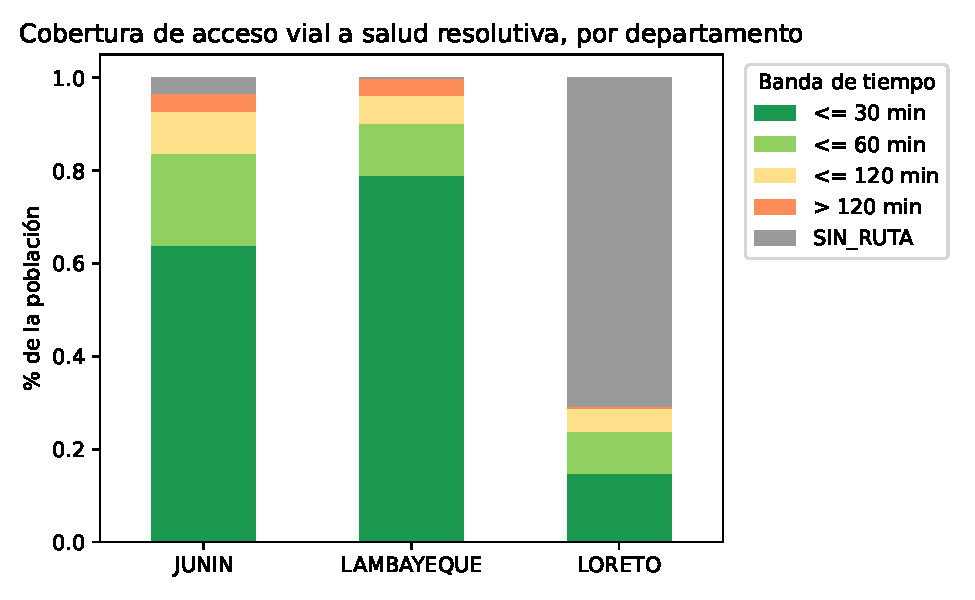
\includegraphics[width=0.8\textwidth]{figures/cobertura_bandas.pdf}
  \caption{Cobertura de acceso vial a salud resolutiva, por departamento.}
  \label{fig:cobertura}
\end{figure}

\begin{table}[H]
\caption{Acceso ponderado por población, por departamento.}
\label{tab:acceso_departamental}
\centering
\resizebox{\textwidth}{!}{%
\begin{tabular}{lrrrr}
\toprule
Departamento & Población & Acceso medio ponderado (min) & Sin ruta (\%) & Centros poblados (muestra) \\
\midrule
LORETO & 1068130 & 35.0 & 89.5 & 1492 \\
JUNIN & 1379934 & 32.9 & 3.6 & 2650 \\
LAMBAYEQUE & 1290617 & 22.7 & 0.7 & 858 \\
\bottomrule
\end{tabular}
}
\end{table}


\subsection{Brechas críticas}
El distrito con peor acceso ponderado es Pampa Hermosa (Loreto, 280
minutos, 61.1\% de sus centros poblados sin ruta). De los 10 peores
distritos, 5 son de Junín, 4 de Lambayeque y 1 de Loreto -- Loreto domina
en la categoría ``sin ruta'' pero no necesariamente en ``tiempo más largo
entre los que sí rutean'', porque los pocos loretanos que logran conectar
a la red suelen estar relativamente cerca de un resolutivo urbano.

\begin{table}[H]
\caption{Los 10 distritos con peor acceso ponderado por población.}
\label{tab:brechas_criticas}
\centering
\resizebox{\textwidth}{!}{%
\begin{tabular}{llrrr}
\toprule
Distrito & Departamento & Acceso (min) & Población & Sin ruta (\%) \\
\midrule
PAMPA HERMOSA & LORETO & 279.9 & 11081 & 61.1 \\
VIZCATAN DEL ENE & JUNIN & 232.5 & 3573 & 18.8 \\
RIO TAMBO & JUNIN & 228.2 & 61259 & 23.8 \\
CAÑARIS & LAMBAYEQUE & 198.0 & 14787 & 10.7 \\
SANTO DOMINGO DE ACOBAMBA & JUNIN & 176.8 & 7776 & 24.1 \\
INCAHUASI & LAMBAYEQUE & 144.2 & 15733 & 0.0 \\
ANDAMARCA & JUNIN & 125.9 & 4536 & 0.0 \\
TENIENTE CESAR LOPEZ ROJAS & LORETO & 117.6 & 6743 & 86.4 \\
OLMOS & LAMBAYEQUE & 113.9 & 41587 & 0.0 \\
SALAS & LAMBAYEQUE & 112.4 & 13056 & 1.5 \\
\bottomrule
\end{tabular}
}
\end{table}


\subsection{Desigualdad de acceso}
El coeficiente de Gini del tiempo de acceso ponderado por población es
0.633 para los tres departamentos combinados. Por departamento: Lambayeque
0.647, Junín 0.632, Loreto 0.518 -- Loreto es, contra-intuitivamente, el
\emph{menos} desigual, porque su población rutea­ble está mayormente
concentrada cerca de las pocas ciudades conectadas (Iquitos, Nauta), y su
población más aislada queda fuera del cálculo (``sin ruta'', no
``desigual pero conectada'').

\begin{figure}[H]
  \centering
  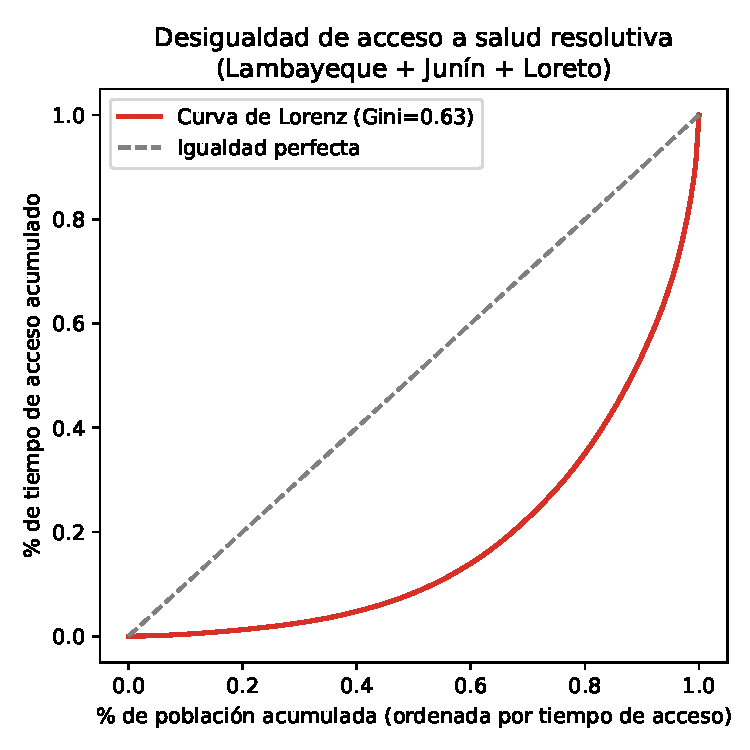
\includegraphics[width=0.65\textwidth]{figures/curva_lorenz.pdf}
  \caption{Curva de Lorenz del tiempo de acceso ponderado por población.}
  \label{fig:lorenz}
\end{figure}

\subsection{Urbano vs. rural}
El acceso ponderado promedio es 12.1 minutos en zonas urbanas contra 29.0
minutos en rurales -- 2.4x más lento. La tasa de ``sin ruta'' también es
mayor en zonas rurales (28.9\% vs. 18.3\%).

\subsection{Cruce con densidad poblacional}
La correlación entre el logaritmo de la densidad poblacional distrital y el
tiempo de acceso ponderado es $r=-0.56$: a mayor densidad, menor tiempo de
acceso. Esta relación es \textbf{correlacional, no causal} -- densidad y
acceso comparten causas comunes (geografía, historia de inversión pública
en infraestructura) que este análisis no puede aislar. No se puede concluir
que ``densificar'' un distrito mejoraría su acceso.

\subsection{Comparación entre modos}
La mediana del ratio tiempo-a-pie/tiempo-en-auto al resolutivo más cercano
es 10.3x; en bicicleta, 3.3x -- ambos ratios subieron frente a una versión
preliminar de este análisis porque el tiempo en auto bajó al corregir el
bug de velocidades (Sección 3.2), no porque caminar o pedalear se haya
vuelto más lento. El establecimiento resolutivo más cercano \emph{cambia}
entre auto y a pie en el 11.8\% de los puntos con ruta válida en ambos
modos -- la mayoría de la población tiene el mismo resolutivo más cercano
sin importar el modo, pero para 1 de cada 8.5 no es así.

\begin{figure}[H]
  \centering
  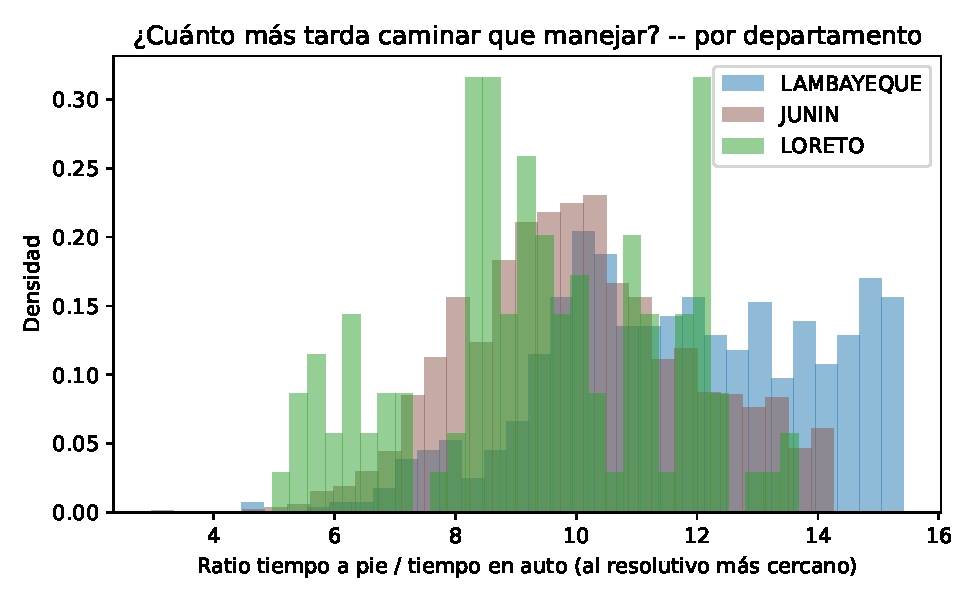
\includegraphics[width=0.8\textwidth]{figures/ratio_pie_auto.pdf}
  \caption{Distribución del ratio tiempo a pie / tiempo en auto, por departamento.}
  \label{fig:ratio}
\end{figure}

\section{Discusión}
\subsection{Distancia en línea recta vs. red vial}
El factor de detour (distancia ruteada / distancia en línea recta) tiene
mediana 1.46 en Junín, contra 1.19 en Lambayeque y 1.19 en Loreto
(Tabla~\ref{tab:detour}). Esto confirma la hipótesis geográfica: el terreno
montañoso de la sierra obliga a caminos mucho más sinuosos que la costa
plana o los ríos/carreteras rectas de la selva baja. Una estimación en
línea recta sin este factor de corrección subestimaría sistemáticamente el
tiempo real en Junín en casi 50\%.

\begin{table}[H]
\caption{Factor de detour (distancia en red / distancia en línea recta), por departamento.}
\label{tab:detour}
\begin{tabular}{lrrrr}
\toprule
Departamento & N pares & Detour mediana & Detour media & Detour p90 \\
\midrule
LAMBAYEQUE & 13632 & 1.19 & 1.23 & 1.45 \\
JUNIN & 66404 & 1.46 & 1.59 & 2.13 \\
LORETO & 900 & 1.19 & 1.23 & 1.44 \\
\bottomrule
\end{tabular}
\end{table}


\subsection{Por qué costa, sierra y selva no se comportan igual}
Los tres departamentos fallan de maneras estructuralmente distintas:
Loreto tiene una red vial \emph{fragmentada} (501 de 501+ componentes
conexas en el grafo de auto, la mayor con solo 58\% de los nodos) -- gran
parte de su población simplemente no está en ninguna carretera mapeada,
consistente con una economía de transporte fluvial que este pipeline no
modela. Junín tiene una red \emph{conectada pero sinuosa} -- el problema no
es llegar a una carretera, es cuánto serpentea esa carretera por la
montaña. Lambayeque tiene la red más densa y menos problemática de los
tres.

\section{Limitaciones}
\begin{itemize}
  \item \textbf{Tasa de error de RENIPRESS}: 32.9\% de coordenadas nulas en
        el ámbito de estudio, 20.2\% de discrepancia punto-distrito
        declarado (Fase 1) -- no se puede garantizar que el 100\% de los
        establecimientos restantes tengan coordenada perfecta.
  \item \textbf{Cobertura de OSM sesgada hacia zonas urbanas}; la Amazonía
        depende de transporte fluvial que este pipeline no modela en
        absoluto -- el 89.5\% de centros poblados (70.8\% de la población)
        ``sin ruta'' en Loreto es, en parte real (no hay carretera) y en
        parte artefacto de esa omisión.
  \item Se asume que un establecimiento listado como \texttt{ACTIVO} está
        realmente operativo y con personal -- RENIPRESS no lo garantiza.
  \item No se modela disponibilidad de ambulancia ni tiempo de atención
        previo al traslado (triage, alistamiento).
  \item \textbf{Muestreo de demanda}: se analizó una muestra estratificada
        por distrito de 5,000 de 13,358 centros poblados ($\sim$37\% de
        retención). Se corrigió el peso muestral para que los totales de
        población sean correctos, pero distritos con pocos centros
        poblados en la muestra tienen una estimación más ruidosa de su
        acceso ponderado -- los valores extremos en
        Tabla~\ref{tab:brechas_criticas} (basados en 1-3 centros poblados
        muestreados por distrito en varios casos) deben leerse con esa
        cautela.
  \item \textbf{Grafo vial no dirigido} (sin restricciones de sentido
        único); velocidades por tipo de vía son un supuesto, no vienen de
        \texttt{maxspeed} real.
  \item \textbf{Población por centro poblado} es un reparto uniforme de la
        población distrital (SIGMED no publica población por centro
        poblado), no la distribución real -- un centro poblado capital
        probablemente concentra más población real que la que este reparto
        le asigna.
  \item Límites distritales de una fuente comunitaria, no el shapefile
        oficial de INEI/IDEP -- se detectó al menos un error de codificación
        de texto en esa capa (no afectó las métricas, que usan SIGMED).
\end{itemize}

\section{Conclusiones y recomendaciones}
La brecha de acceso a salud resolutiva en estos tres departamentos no es
uniforme ni en magnitud ni en causa. En Loreto, el problema dominante es de
\textbf{conectividad} (no hay ruta, no ``la ruta es larga'') -- ahí
priorizar nuevos establecimientos resolutivos por vía terrestre tiene
retorno limitado si la población objetivo no está conectada a ninguna
carretera; probablemente valga más invertir en transporte fluvial de
emergencia o telemedicina/estabilización remota. En Junín, el problema es
de \textbf{sinuosidad del terreno} -- ahí sí un nuevo resolutivo bien
ubicado (el simulador de escenarios del dashboard permite probar
candidatos I-3/I-4 concretos) puede reducir sustancialmente el tiempo
ponderado. Pampa Hermosa (Loreto) y Río Tambo (Junín) son los candidatos
más claros para intervención prioritaria, con las salvedades de tamaño de
muestra ya señaladas.

\section*{Referencias}
\begin{itemize}
  \item RENIPRESS/SUSALUD -- Registro Nacional de IPRESS. MINSA-SUSALUD.
  \item SIGMED -- Sistema de Información Geográfica Educativa, MINEDU.
  \item Geofabrik GmbH -- extracto OSM de Perú, datos © OpenStreetMap
        contributors, licencia ODbL.
  \item INEI -- Censos Nacionales 2017: XII de Población, VII de Vivienda.
  \item \texttt{juaneladio/peru-geojson} y \texttt{geodir/ubigeo-peru}
        (repositorios comunitarios de datos abiertos de Perú, GitHub).
\end{itemize}

\end{document}
